\documentclass[
  a4paper,uplatex,dvipdfmx,9pt,
  xcolor = {dvipsnames,svgnames},
  hyperref ={colorlinks=true,citecolor=Navy,linkcolor=NavyBlue,urlcolor=purple}
]{beamer}
\renewcommand{\baselinestretch}{1.4}

% ---refer `texdoc xcolor' at the command line---

% ---Display \subsubsection at the Index
% \setcounter{tocdepth}{3}

% ---Setting about the geometry of the document----
% \usepackage{a4wide}
% \pagestyle{empty}

% ---Physics and Math Packages---
\usepackage{amssymb,amsfonts,amsthm,mathtools}
\usepackage{physics,braket,bm}

% ---underline---
\usepackage{ulem}

% ---cancel---
\usepackage{cancel}

% --- surround the texts or equations
% \usepackage{fancybox,ascmac}

% ---settings of theorem environment---
% \usepackage{amsthm}
% \theoremstyle{definition}

% ---settings of proof environment---
% \renewcommand{\proofname}{\textbf{証明}}
% \renewcommand{\qedsymbol}{$\blacksquare$}

% ---Ignore the Warnings---
\usepackage{silence}
\WarningFilter{latexfont}{Some font shapes,Font shape}
\ExplSyntaxOn
\msg_redirect_name:nnn{hooks}{generic-deprecated}{none}
\ExplSyntaxOff

% ---Insert the figure (If insert the `draft' at the option, the process becomes faster.)---
\usepackage{graphicx}
% \usepackage{subcaption}

% ----Add a link to a text---
\usepackage{url,hyperref}
\usepackage{xcolor}
\usepackage{pxjahyper}

% ---Tikz---
\usepackage{tikz,pgf,pgfplots,circuitikz}
\pgfplotsset{compat=1.15}
\usetikzlibrary{intersections,arrows.meta,angles,calc,3d,decorations.pathmorphing,positioning}

% ---Add the section number to the equation, figure, and table number---
\makeatletter
   \renewcommand{\theequation}{\thesection.\arabic{equation}}
   \@addtoreset{equation}{section}
   
   \renewcommand{\thefigure}{\thesection.\arabic{figure}}
   \@addtoreset{figure}{section}
   
   \renewcommand{\thetable}{\thesection.\arabic{table}}
   \@addtoreset{table}{section}
\makeatother

% ---enumerate---
% \renewcommand{\labelenumi}{$\arabic{enumi}.$}
% \renewcommand{\labelenumii}{$(\arabic{enumii})$}

% ---beamer settings---
\usefonttheme{professionalfonts}
% \usefonttheme{serif}
\usecolortheme{seahorse}
\setbeamercolor{structure}{fg=Turquoise}
\setbeamercolor{local structure}{fg=Turquoise}
\setbeamertemplate{itemize item}[ball]
\setbeamertemplate{enumerate item}[circle]
\setbeamercolor{bibliography entry author}{fg=black}
\setbeamercolor{bibliography item}{fg=black}
\setbeamercolor{alerted text}{fg=RoyalBlue}
\setbeamertemplate{frametitle continuation}{}
\setbeamertemplate{footline}[frame number]
\setbeamertemplate{navigation symbols}{} 

% ---tcolorbox---
\usepackage{tcolorbox}
\tcbuselibrary{raster,skins}
\newtcolorbox{boxmine}[2][]{enhanced,
colframe=RoyalBlue!40!white,
colback=RoyalBlue!10!white,
coltitle=black,
drop fuzzy shadow, title={#2}
,#1}

% ---Fonts---
\renewcommand{\familydefault}{\sfdefault}
\renewcommand{\kanjifamilydefault}{\gtdefault}
% \usepackage{newtxmath}
\mathversion{bold}

% ---
\usepackage{usebib}
\newbibfield{author} 
\newbibfield{year} 
\newbibfield{journal} 
\newbibfield{doi} 
\bibinput{hoge}

\makeatletter
\newcommand*{\journal}{\begingroup\@makeother\#\@mylink}
\newcommand*{\@mylink}[1]{\href{http://dx.doi.org/\usebibentry{#1}{doi}}{\usebibentry{#1}{journal}}\endgroup} 
\makeatother

\newcommand*{\citefone}[2]{
  \begin{tikzpicture}[remember picture, overlay]
    \node[anchor=north east, align=left] at ($(current page.north east)-(0,0.0)$){
    {\tiny
      \cite{#1}
      #2,
      \journal{#1}
      (\usebibentry{#1}{year}).
    }
    };
  \end{tikzpicture}
}

\newcommand*{\citeftwo}[4]{
  \begin{tikzpicture}[remember picture, overlay]
    \node[anchor=north east, align=left] at ($(current page.north east)-(0,0.0)$){
    {\tiny
      \cite{#1}
      #2,
      \journal{#1}
      (\usebibentry{#1}{year}).
    }
    \\[-2.4ex]
    {\tiny
      \cite{#3}
      #4,
      \journal{#3}
      (\usebibentry{#3}{year}).
    }
    };
  \end{tikzpicture}
}

\newcommand*{\citefthree}[6]{
  \begin{tikzpicture}[remember picture, overlay]
    \node[anchor=north east, align=left] at ($(current page.north east)-(0,0.0)$){
    {\tiny
      \cite{#1}
      #2,
      \journal{#1}
      (\usebibentry{#1}{year}).
    }
    \\[-2.4ex]
    {\tiny
      \cite{#3}
      #4,
      \journal{#3}
      (\usebibentry{#3}{year}).
    }
    \\[-2.4ex]
    {\tiny
      \cite{#5}
      #6,
      \journal{#5}
      (\usebibentry{#5}{year}).
    }
    };
  \end{tikzpicture}
}



% ---Title---
\title{
  卒論\ 中間発表\ 2
  \\
  {\LARGE
    磁化トーラス上にコンパクト化した
    \\
    超対称模型におけるモジュライ固定
  }
}
\author{宮根 一樹}
\date{2024年1月16日}

\begin{document}

\begin{frame}
  \titlepage
\end{frame}

\setbeamertemplate{section in toc}[circle]
\setbeamertemplate{subsection in toc}[ball]
\begin{frame}[allowframebreaks]
  \frametitle{目次}
  \tableofcontents
\end{frame}


\section{イントロダクション}

\begin{frame}
  \frametitle{\thesection\ \secname}

  素粒子標準模型
  \begin{itemize}
    \item 
    実験でよく結果が確認されている
    \item 
    $SU(3)_{C}\times SU(2)_{L}\times U(1)_{Y}$のゲージ理論
    \item 
    物質場は3世代
    \item 
    物質の左右が非対称$\rightarrow$カイラルな理論
  \end{itemize}

  \vspace{10pt}

  \begin{columns}[t]    
    \begin{column}{0.4\textwidth} 
      標準模型の問題点
      \begin{itemize}
        \item 
        重力が含まれていない
        \item 
        世代間の質量階層性
      \end{itemize}
      など    
    \end{column}
    \begin{column}{0.4\textwidth}  
      $\longrightarrow$高次元時空モデルの考案
    
      \begin{itemize}
        \item[\uline{\textcolor{black}{e.g.}}]    
        超弦理論    
        \item 
        重力を含む
        \item 
        10次元で無矛盾な理論
      \end{itemize}
    \end{column}
  \end{columns}

  \vspace{10pt}

  現実的なモデルを得るためには
  \begin{itemize}
    \item 
    余剰次元を観測できないほどにコンパクト化
    \item 
    カイラリティやゲージ群,質量や結合定数などを再現
  \end{itemize}

\end{frame}

\begin{frame}
  \frametitle{\thesection\ \secname}
  
  \uline{コンパクト化}

  \begin{itemize}
    \item 
    超弦理論では10次元時空(4次元ミンコフスキー $+$ \uwave{6次元余剰次元})
    \item 
    その低エネルギー有効理論は10次元の場の理論
  \end{itemize}

  \vspace{5pt}

  \begin{itemize}
    \item [\textcolor{black}{\uline{e.g.}}]
    ヤン・ミルズ理論の結合定数(詳しい理論は後述)

    \begin{align}
      &\hspace{-1cm}
      \int\dd^{10}X
      \sqrt{-G}\frac{1}{g^2}\text{Tr}\left[ -\frac{1}{4}F^{MN}F_{MN} \right]
      \nonumber
      \\
      &=
      \int\dd^{4}x
      \underbrace{
        \left(  
          \int\dd^{6}y
          \sqrt{-G}\frac{1}{g^2}
        \right)
      }_{\equiv 1/g_{4D}^2}
      \text{Tr}\left[ -\frac{1}{4}F^{\mu\nu}F_{\mu\nu} \right]
      +
      (\cdots)
      \nonumber
    \end{align}
    
    $\longrightarrow$
    \textcolor{DarkMagenta}{余剰次元の形}が\textcolor{DarkGreen}{4次元のゲージ結合定数など}を決定
    
  \end{itemize}

\end{frame}

\begin{frame}
  \frametitle{\thesection\ \secname}
    
  \begin{itemize}
    \item 
    10次元時空の計量
    \begin{equation}
      G_{MN}(x)
      =
      \begin{pmatrix}
        g_{\mu\nu}(x) & * \\
        * & G_{mn}(x)
      \end{pmatrix}
      \nonumber
    \end{equation}
    \item 
    $G_{mn}(x)$:4次元でのスカラー場\ (\textcolor{DarkMagenta}{モジュライ}という)
    \item 
    モジュライの真空期待値はポテンシャルで決定
    $\longrightarrow$
    \textcolor{DarkMagenta}{モジュライ固定}
  \end{itemize}

  \begin{columns}[t]    
    \begin{column}{0.49\textwidth} 
      \begin{center}
        余剰次元の形はダイナミカルな場$G_{mn}(x)$

        \vspace{5pt}

        $\downarrow$

        \vspace{5pt}

        真空期待値になる$\ev*{G_{mn}}$
      \end{center}
    \end{column}
    \begin{column}{0.4\textwidth}  
      \begin{figure}[ht]
        \centering
        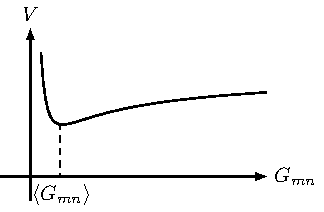
\includegraphics[keepaspectratio,width=0.8\linewidth]{fig/intro_potential/intro_potential.pdf}         
      \end{figure}
    \end{column}
  \end{columns}

\end{frame}


\begin{frame}
  \frametitle{\thesection\ \secname}
  
  \citefthree{Abe_SuperfieldDescription_2012}{H. Abe, T. Kobayashi, H. Ohki, and K. Sumita}{Abe_AhlerModuli_2017}{H. Abe, T. Kobayashi, K. Sumita, and S. Uemura}{Abe_ModuliStabilization_2007a}{H. Abe, T. Higaki, T. Kobayashi, and Y. Omura}
    
  \begin{boxmine}{先行研究}
    \begin{itemize}
      \item 
      標準模型が再現されるようなモデル$\rightarrow$\cite{Abe_SuperfieldDescription_2012,Abe_AhlerModuli_2017}
      \item 
      モジュライ固定ができているモデル$\rightarrow$\cite{Abe_ModuliStabilization_2007a}
    \end{itemize}
  \end{boxmine}
    
  \begin{boxmine}{卒業研究}
    標準模型が再現されうるモデルでのモジュライ固定は?
  \end{boxmine}

\end{frame}


\section{磁化トーラス模型と\texorpdfstring{$D$}{D}-termポテンシャルの解析}

\subsection{超対称ヤン・ミルズ理論}

\begin{frame}
  \frametitle{\thesection.\thesubsection\ \subsecname}  

  \citeftwo{Arkani-Hamed_HigherDimensional_2002}{N. Arkani-Hamed, T. Gregoire, and J. Wacker}{Abe_SuperfieldDescription_2012}{H. Abe, T. Kobayashi, H. Ohki, and K. Sumita}

  \vspace*{-0.7cm}

  \uline{10次元超対称ヤン・ミルズ理論(10D SYM)}

  \begin{itemize}
    \item 
    作用
    \begin{equation}
      S
      =
      \int\dd^{10}X\sqrt{-G}
      \frac{1}{g^2}\text{Tr}\ \left[
      -\frac{1}{4}F^{MN}F_{MN}+\frac{i}{2}\bar{\lambda}\Gamma^{M}D_{M}\lambda
      \right]
      \label{action_10DSYM}
      \nonumber
    \end{equation}
    \item 
    あらわれている記号
    \begin{align}
      &
      g:\text{結合定数}
      ,\
      G_{MN}:\text{10次元での計量\ $M,N=0,1,\cdots,9$}
      \nonumber
      \\
      &
      F_{MN}
      =
      \partial_{M}A_{N}-\partial_{N}A_{M}
      -
      i[A_{M},A_{N}]
      \text{:場の強度}
      ,
      \nonumber
      \\
      &
      D_{M}\lambda
      =
      \partial_{M}\lambda
      -
      i[A_{M},\lambda]
      \text{:共変微分,これで局所ゲージ不変に}
      ,
      \nonumber
      \\
      &
      \lambda
      \text{:マヨラナ・ワイル\ $\rightarrow$\ 10次元で中性$+$カイラリティーが正}
      .
      \nonumber
    \end{align}
    \item 
    ベクトル場$A_{M}$,スピノル場$\lambda$はそれぞれゲージ群のアジョイント表現の添え字をもつ
    
    $\longrightarrow$トレース$\text{Tr}$はその行列の添え字について

    \item 
    ボゾンとフェルミオンの対称性(\textcolor{DarkMagenta}{超対称性})をもつ
  \end{itemize}
\end{frame}

\subsection{トーラスコンパクト化}

\begin{frame}
  \frametitle{\thesection.\thesubsection\ \subsecname}

  \citeftwo{Arkani-Hamed_HigherDimensional_2002}{N. Arkani-Hamed, T. Gregoire, and J. Wacker}{Abe_SuperfieldDescription_2012}{H. Abe, T. Kobayashi, H. Ohki, and K. Sumita}

  \begin{itemize}
    \item 
    10次元ミンコフスキー空間$(x^{\mu},y^{m})\ \mu=0,\cdots,3,\ m=4,\cdots,9$
    \item 
    トーラス$T^{2}$を実現する境界条件:
    \begin{equation}
      y^{2i+2}\sim y^{2i+2}+2\ \&\ y^{2i+3}\sim y^{2i+3}+2\quad (i=1,2,3)
      \nonumber      
    \end{equation}
    \begin{figure}[ht]
      \centering        
      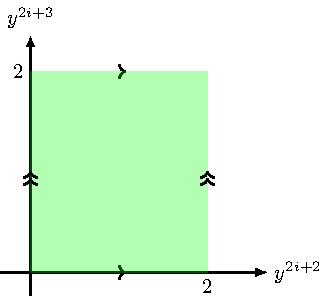
\includegraphics[keepaspectratio,width=0.3\linewidth]{fig/torus/torus1.pdf}       
    \end{figure}
    \item 
    余剰次元の形
    \begin{equation}
      g^{(i)}
      =
      (2\pi R_{i})^2
      \begin{pmatrix}
        1 & 0 \\
        0 & 1
      \end{pmatrix}
      \text{:トーラスの計量}
      \nonumber
    \end{equation}
    $\longrightarrow$ $ R_{i}$が余剰次元の形を決定
  \end{itemize}

\end{frame}

\begin{frame}
  \frametitle{\thesection.\thesubsection\ \subsecname}

  \citefthree{Arkani-Hamed_HigherDimensional_2002}{N. Arkani-Hamed, T. Gregoire, and J. Wacker}{Abe_SuperfieldDescription_2012}{H. Abe, T. Kobayashi, H. Ohki, and K. Sumita}{Abe_AhlerModuli_2017}{H. Abe, T. Kobayashi, K. Sumita, and S. Uemura}

  \begin{itemize}
    \item 
    余剰次元方向の座標$y^{m}$を複素座標$z^{i}$に取りなおし
    \begin{center}
      $
      (y_{4},y_{5})
      \rightarrow
      (z_{1},\bar{z}_{1})
      ,\ 
      (y_{6},y_{7})
      \rightarrow
      (z_{2},\bar{z}_{2})
      ,\ 
      (y_{8},y_{9})
      \rightarrow
      (z_{3},\bar{z}_{3})
      $    
    \end{center}
    例えば,座標やゲージ場
    \begin{equation}      
      \left\{
        \begin{alignedat}{1}
          z^{1}
          &\equiv
          \frac{1}{2}(y^4+i y^5)
          \\
          \tilde{A}_{1}
          &\equiv
          iA_{4}+A_{5}
        \end{alignedat}
      \right.
      \quad
      \text{
        $z^{2},z^{3}$や$\tilde{A}_{2},\tilde{A}_{3}$も同様に定義
      }
      \nonumber
    \end{equation}
    以後,$\tilde{A}_{i}$を$A_{i}$と書く
    \item
    $z^{i}$での境界条件:
    $
      z^{i} \sim z^{i}+1
      \ \&\ 
      z^{i} \sim z^{i}+i      
      \nonumber
    $
    \item 
    独立なトーラス$T^2$が3つ$\longrightarrow T^2\times T^2\times T^2$
  \end{itemize}

  \pause

  \begin{equation}
    \mathcal{A}^{(i)}
    =
    (2\pi R_{i})^2
    \text{
      :$i$番目のトーラスの面積
    }
    \nonumber
  \end{equation}

  \begin{center}
    \textcolor{DarkRed}{
      $\ev*{T_{i}}\equiv\mathcal{A}^{(i)}$となるようなダイナミカルな場$T_{i}$をモジュライとよぶ
    }    
  \end{center}

\end{frame}

\subsection{\texorpdfstring{$D$-term}{D-term}ポテンシャル}

\begin{frame}
  \frametitle{\thesection.\thesubsection\ \subsecname}

  \citefone{Abe_SuperfieldDescription_2012}{H. Abe, T. Kobayashi, H. Ohki, and K. Sumita}

  \vspace*{-0.8cm}

  \begin{itemize}
    \item 
    \hyperlink{action_10DSYM}{10D SYMの作用}から
    \begin{equation}
      V^{(D)}
      \equiv
      \text{Tr}
      \left[  
        \left(  
          \frac{1}{\mathcal{A}^{(1)}}
          F_{45}
          +
          \frac{1}{\mathcal{A}^{(2)}}
          F_{67}
          +
          \frac{1}{\mathcal{A}^{(3)}}
          F_{89}
        \right)^2
      \right]
      \times
      \prod_{i=1,2,3}\mathcal{A}^{(i)}
      \nonumber
    \end{equation}
    \begin{center}
      今回考えるポテンシャル$\longrightarrow$
      \textcolor{DarkRed}{$D$-termポテンシャル}
      
      (ポテンシャルにはまだ別の項が$\rightarrow$次の真空期待値で消えるので無視)
    \end{center}

    \vspace{10pt}

    \item 
    ベクトル場の真空期待値
    \begin{equation}
      \ev*{A_{i}}_{ab}
      \equiv
      \pi M_{ab}^{(i)}\bar{z}^{i}
      ,\ 
      M_{ab}^{(i)}
      =
      \begin{pmatrix}
        M_{1}^{(i)} & 0 \\
        0 & M_{2}^{(i)}
      \end{pmatrix}
      \nonumber
    \end{equation}
    \begin{itemize}
      \item 
      $M_{a}^{(i)}$は整数
      \item 
      $M^{(i)}$は$i$番目のトーラス上の磁場
      
      \hspace{1cm}
      $\rightarrow\ F_{45}=\pi M^{(1)},F_{67}=\pi M^{(2)},F_{89}=\pi M^{(3)}$
    \end{itemize}

  \end{itemize}

\end{frame}

\begin{frame}
  \frametitle{\thesection.\thesubsection\ \subsecname}

  \begin{itemize}
    \item 
    背景磁場があるときの$D$-termポテンシャル

    \hspace*{3cm}
    $\rightarrow$
    $\mathcal{A}^{(i)}$をダイナミカルな場$T_{i}$に
    \begin{equation}
      V^{(D)}
      =
      \sum_{a=1,2}
      \left(  
        \sum_{i=1,2,3}
        \frac{\pi M_{a}^{(i)}}{T_{i}}
      \right)^2
      \times
      \prod_{i=1,2,3}T_{i}
      \nonumber
    \end{equation}
    \item 
    真空期待値$\ev*{T_{i}}$が満たす条件:
    \begin{equation}
      \partial_{T_{i}}V^{(D)}=0
      \quad
      (\text{for}\ i=1,2,3)
      \longrightarrow
      \sum_{i=1,2,3}
      \frac{\pi M_{a}^{(i)}}{\ev*{T_{i}}}
      =
      0
      \quad
      (a=1,2)
      \label{SUSY_cond}
      \nonumber
    \end{equation}

    \item 
    $V^{(D)}$を真空期待値$\ev*{T_{i}}$のまわりで展開
    \begin{equation}
      V^{(D)}
      =
      V^{(D)}
      \left.\vphantom{\frac{1}{2}}\right|_{0}
      +
      \frac{1}{2}
      \underbrace{
        \partial_{T_{r}}\partial_{T_{r'}}V^{(D)}
        \left.\vphantom{\frac{1}{2}}\right|_{0}
      }_{\equiv V_{rr'}}
      \delta T_{r}\delta T_{r'}
      +
      \mathcal{O}(\delta T^3)
      \nonumber
    \end{equation}
    \begin{center}
      $\delta T_{r}\equiv T_{r}-\ev*{T_{r}}$\ \&\ $\cdot\left.\vphantom{\frac{1}{2}}\right|_{0}$は真空期待値を代入
    \end{center}

    \vspace{5pt}

    $\longrightarrow$ $\delta T_{r}$の2次の項を対角化
    \qquad
    \textcolor{DarkMagenta}{$V_{rr'}$の固有値はモジュライの質量}
  \end{itemize}

\end{frame}

\begin{frame}
  \frametitle{\thesection.\thesubsection\ \subsecname}

  \vspace*{-0.6cm}

  \begin{columns}[t]    
    \begin{column}{0.49\textwidth} 
      \begin{center}
        対角化を実行$\rightarrow$対角化行列を$P$
        \begin{gather}
          \begin{pmatrix}
            0 & & \\
            & m_{2}^2 & \\
            & & m_{3}^2
          \end{pmatrix}
          \equiv
          P^{T}(V_{rr'})P
          \nonumber
        \end{gather}
        $m_{2},m_{3}$はモジュライの質量
        
        ($V_{rr'}$の固有値)
      \end{center}
    \end{column}
    \begin{column}{0.4\textwidth}  
      \begin{figure}[ht]
        \centering
        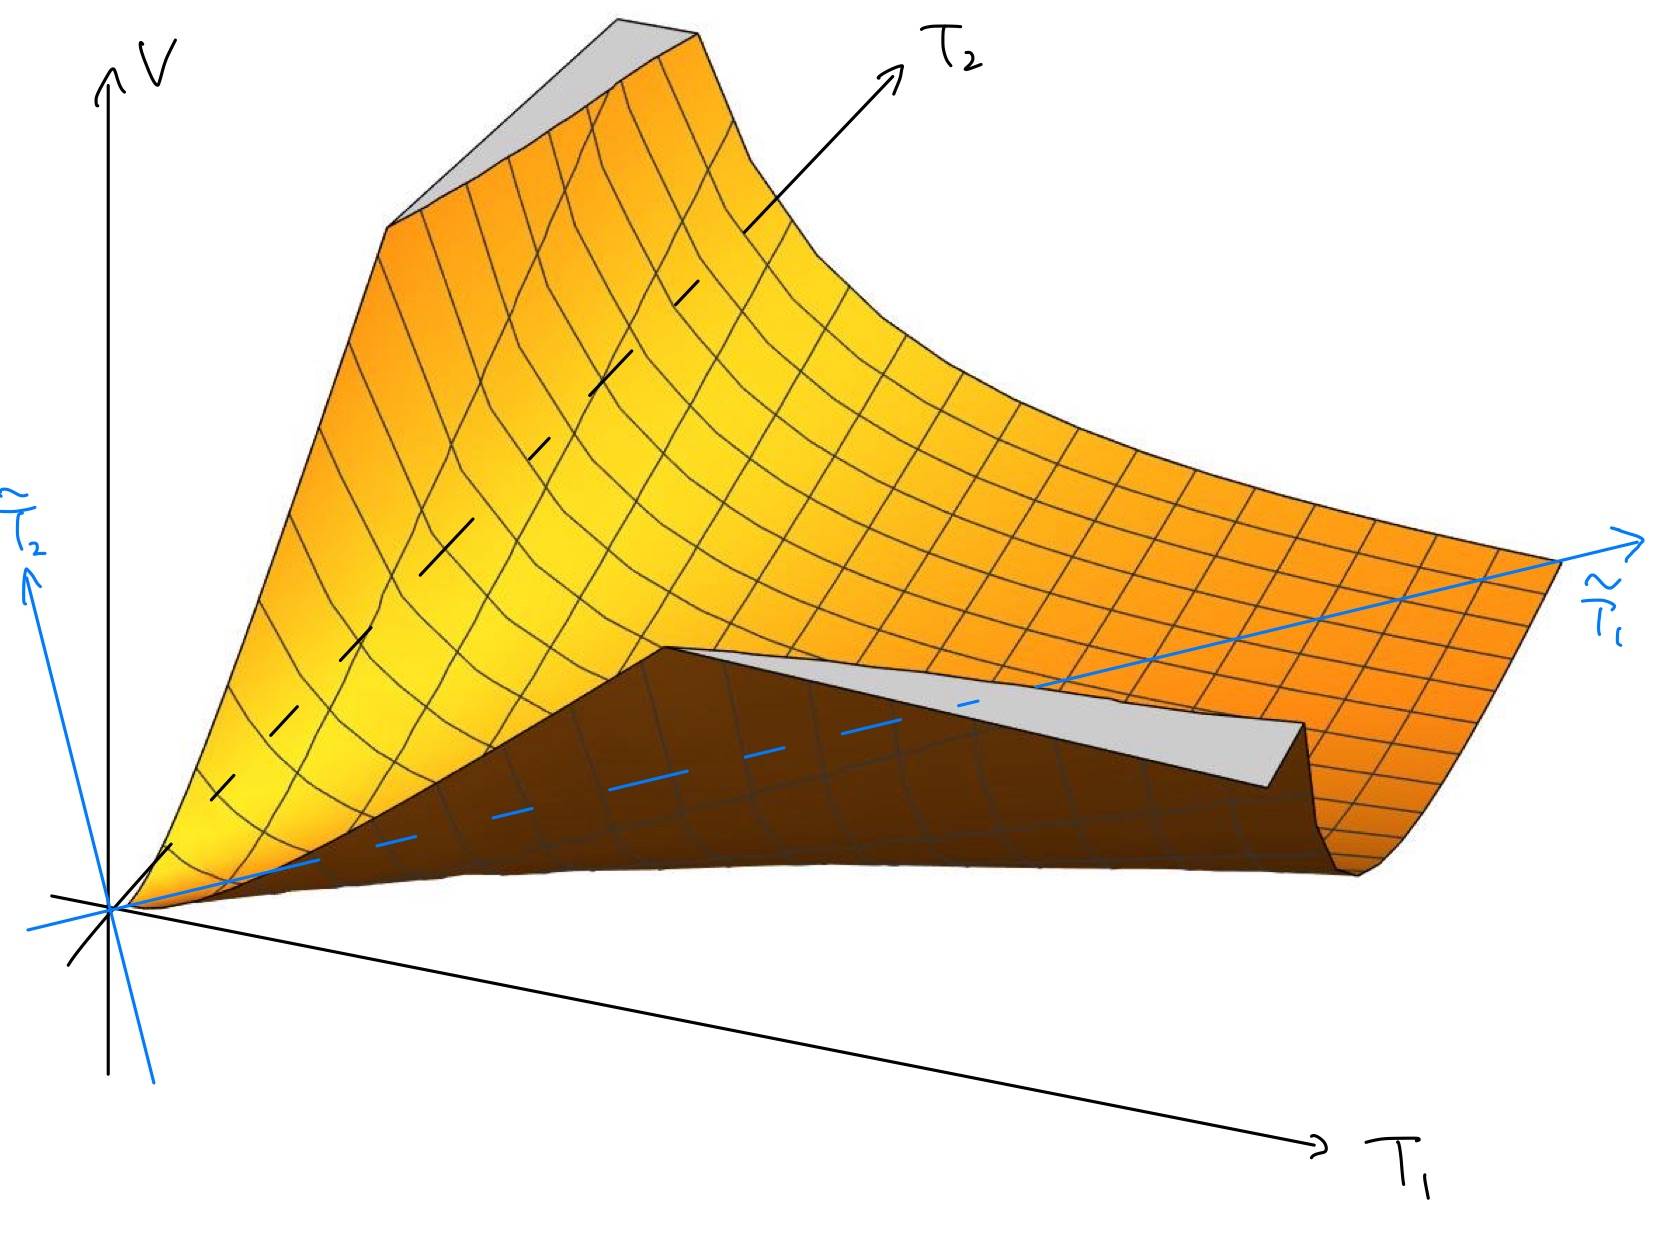
\includegraphics[keepaspectratio,width=0.8\linewidth]{fig/dterm_potential.jpg}         
      \end{figure}
    \end{column}
  \end{columns}

  \vspace{10pt}

  \begin{itemize}
    \item 
    対角化された基底$\delta \tilde{T}_{i}(=\sum(P^{T})_{ij}\delta T_{j})$
    \begin{equation}
      \frac{1}{2}
      V_{rr'}
      \delta T_{r}\delta T_{r'}
      \rightarrow
      \frac{1}{2}m_{2}^2 \delta \tilde{T}_{2}^2
      +
      \frac{1}{2}m_{3}^2 \delta \tilde{T}_{3}^2
      \nonumber
    \end{equation}
    \item 
    固有値が0の方向は$\delta \tilde{T}_{1}\equiv\tilde{T}$
    (以後,揺らぎをそのまま場とみなす)
    \item 
    パラメター
    \begin{itemize}
      \item 
      $M_{a}^{(i)}$:磁場6つ$\rightarrow$標準模型を再現するような値
      \item 
      $\ev*{T_{1}}$:(対角化前の基底の)モジュライの真空期待値$\rightarrow$\textcolor{DarkMagenta}{超重力理論で値を決定}
    \end{itemize}
  \end{itemize}

\end{frame}


\section{\texorpdfstring{$F$}{F}-termポテンシャルとモジュライ固定}

\subsection{超重力理論とポテンシャル}

\begin{frame}
  \frametitle{\thesection.\thesubsection\ \subsecname}

  \citefone{Abe_SuperfieldDescription_2012}{H. Abe, T. Kobayashi, H. Ohki, and K. Sumita}

  \vspace*{-0.7cm}

  \begin{boxmine}{今後の動機}
      \begin{center}
        $D$-termでは残りのモジュライの真空期待値$\ev*{T_1}$を決定できない

        {\LARGE $\downarrow$}

        4次有効理論のポテンシャルで決定
      \end{center}
  \end{boxmine}

  \vspace{10pt}

  \uline{4次元超重力理論}
  \begin{itemize}
    \item 
    \textcolor{DarkRed}{超対称性}によって,ポテンシャルが強く制限

    $\rightarrow$
    スーパーポテンシャル$W$,ケーラーポテンシャル$K$
    \begin{equation}
      \left\{
        \begin{alignedat}{1}
          W
          &=
          w_{0}
          -
          \sum_{r}
          A_{r}
          e^{-a_{r}T_{r}}
          -
          \sum_{r}B_{r}e^{-b_{r}T_{r}}
          X
          \\
          K
          &=
          -
          \sum_{r}\ln (T_{r}+\bar{T}_{r})
          +
          |X|^2
        \end{alignedat}
      \right.
      \nonumber
    \end{equation}
    \item 
    $T_{r}\ (r=1,2,3)$はモジュライ.$X$は複素スカラー場.
    \item 
    $w_{0},A_{r},a_{r},B_{r},b_{r}$は,\textcolor{DarkGreen}{背景理論}で決まってくる実数パラメター.
  \end{itemize}

\end{frame}

\subsection{モジュライ固定の方法}

\begin{frame}
  \frametitle{\thesection.\thesubsection\ \subsecname}
  
  \citeftwo{Abe_ModuliStabilization_2007a}{H. Abe, T. Higaki, T. Kobayashi, and Y. Omura}{Abe_MoreFterm_2007a}{H. Abe, T. Higaki, and T. Kobayashi}

  \begin{tikzpicture}[remember picture, overlay]
    \node[anchor=north east, align=left] at ($(current page.north east)-(0,5.4)$){
    {
      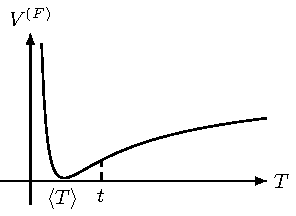
\includegraphics[keepaspectratio,width=3.3cm]{fig/reference_point/reference_point.pdf}       
    }
    };
  \end{tikzpicture}

  \vspace*{-1.5cm}

  \uline{一般論}

  \begin{itemize}
    \item 
    スーパーポテンシャル$W$とケーラーポテンシャル$K$

    \hspace{1cm}$\longrightarrow$スカラーポテンシャル(\textcolor{DarkRed}{$F$-termポテンシャル})
    \begin{gather}
      V^{(F)}
      \equiv
      e^{K}
      (
        K^{I\bar{J}}(D_{I}W)(D_{\bar{J}}\bar{W})
        -
        3|W|^2
      )
      \nonumber
      \\
      D_{I}W
      \equiv
      W_{I}+K_{I}W
      \quad
      (I=X,T)
      \nonumber
    \end{gather}
    \begin{center}
      $f_{I}\equiv\partial_{I}f$,$K^{I\bar{J}}$は$K_{I\bar{J}}$の逆行列      
    \end{center}
    \item 
    $V^{(F)}$の最小値を実現する$T,X$は?

    \hspace{2cm}$\longrightarrow$
    その点にモジュライ$T$が固定
  
    \item 
    ポテンシャルの最小をどのように特定するか?
  
    \begin{itemize}
      \item 
      解析的には難しい
      $\longrightarrow$
      \textcolor{DarkRed}{参照点}を利用すると解析的に
      \item 
      \textcolor{DarkMagenta}{超対称性が保たれる点}がポテンシャルの最小になりやすい
    \end{itemize}
  \end{itemize}
\end{frame}


\begin{frame}
  \frametitle{\thesection.\thesubsection\ \subsecname}

  \citefone{Abe_ModuliStabilization_2007a}{H. Abe, T. Higaki, T. Kobayashi, and Y. Omura}

  \begin{itemize}
    \item 
    参照点$(t,x)$
    \begin{equation}
      D_{T}W
      \left.\vphantom{\frac{1}{2}}\right|_{0}
      =0
      ,\ 
      V_{X}^{(F)}
      \left.\vphantom{\frac{1}{2}}\right|_{0}
      =0
      \quad
      (
        \text{
          $\left.\cdot\hspace{1pt}\right|_{0}$は$(T,X)=(t,x)$の代入
        }
      )
      \nonumber
    \end{equation}
    \begin{center}
      ($D_{T}W=0\longrightarrow$超対称性が保たれている)
    \end{center}
    \item 
    ポテンシャル$V^{(F)}$を参照点からの揺らぎ$\delta T,\delta X$で展開
    \begin{align}
      V^{(F)}
      &=
      \textcolor{gray}{
        V^{(F)}      
        \left.\vphantom{\frac{1}{2}}\right|_{0}
        +
      }
      V_{T}^{(F)}
      \left.\vphantom{\frac{1}{2}}\right|_{0}
      \delta T
      +
      V_{\bar{T}}^{(F)}
      \left.\vphantom{\frac{1}{2}}\right|_{0}
      \delta \bar{T}
      \textcolor{gray}{
        +
        V_{X}^{(F)}
        \left.\vphantom{\frac{1}{2}}\right|_{0}
        \delta X
        +
        \cdots
        +
      }
      \nonumber
      \\
      &\hspace{10pt}
      +
      \frac{1}{2}
      V_{TT}^{(F)}
      \left.\vphantom{\frac{1}{2}}\right|_{0}
      \delta T^2
      +
      \frac{1}{2}
      V_{XX}^{(F)}
      \left.\vphantom{\frac{1}{2}}\right|_{0}
      \delta X^2
      +
      \cdots
      +
      \mathcal{O}(\delta T^3, \delta X^3)
      \nonumber
    \end{align}
    \item 
    $V_{\delta T}, V_{\delta \bar{T}}, V_{\delta X}, V_{\delta \bar{X}}=0\longrightarrow$
    $\delta T, \delta \bar{T}, \delta X, \delta \bar{X}$の値を決定
    \begin{center}
      {\LARGE $\downarrow$}
      
      $\displaystyle
        \frac{\delta T}{t}\ll 1
        ,\ 
        \frac{\delta X}{x}\ll 1
      $
      であれば,\textcolor{DarkRed}{参照点}による近似が有効
    \end{center}
  \end{itemize}

\end{frame}



\begin{frame}
  \frametitle{\thesection.\thesubsection\ \subsecname}
  
  \citeftwo{Abe_ModuliStabilization_2007a}{H. Abe, T. Higaki, T. Kobayashi, and Y. Omura}{Abe_MoreFterm_2007a}{H. Abe, T. Higaki, and T. Kobayashi}

  \uline{先行研究}\cite{Abe_MoreFterm_2007a}

  ポテンシャル
  \begin{equation}
    W
    =
    w_{0}
    -
    A
    e^{-aT}
    -
    Be^{-bT}
    X
    ,\ 
    K
    =
    -
    3\ln (\tilde{T}+\bar{\tilde{T}})
    +
    |X|^2
    \nonumber
  \end{equation}
  のパラメターが
  \begin{equation}
    |a|,|b|\sim 4\pi^2
    ,\ 
    A\sim 1
    \quad
    (B,w_{0}\ll 1\text{?})
    \nonumber
  \end{equation}
  \begin{center}
    {\LARGE $\downarrow$}

    $
      \displaystyle
      \ev*{X}
      =
      \sqrt{3}-1
      ,\ 
      \ev*{T}
      =
      \mathcal{O}(1)
    $
  \end{center}
  \begin{equation}
    \frac{\delta T}{t}
    \sim
    \frac{1}{b^3}
    \ll 1
    ,\ 
    \frac{\delta X}{x}
    \sim
    \frac{1}{b^2}
    \ll 1
    \nonumber
  \end{equation}
  \begin{flushright}
    $\longrightarrow$\textcolor{DarkRed}{参照点}による近似が有効    
  \end{flushright}

\end{frame}


\subsection{具体的なモデルへの適用}

\begin{frame}
  \frametitle{\thesection.\thesubsection\ \subsecname}

  \begin{boxmine}{今後の話}
    先行研究を適用
    $\rightarrow$
    決まらなかったモジュライ$\ev*{T_1}$を決定
  \end{boxmine}
  
  \begin{itemize}
    \item 
    \uline{取り扱いたいモデル}

    スーパーポテンシャル$W$,ケーラーポテンシャル$K$
    \begin{equation}
      \left\{
        \begin{alignedat}{1}
          W
          &=
          w_{0}
          -
          \sum_{r}
          A_{r}
          e^{-a_{r}T_{r}}
          -
          \sum_{r}B_{r}e^{-b_{r}T_{r}}
          X
          \\
          K
          &=
          -
          \sum_{r}\ln (T_{r}+\bar{T}_{r})
          +
          |X|^2
        \end{alignedat}
      \right.
      \nonumber
    \end{equation}
    \item 
    $T_{r}\rightarrow\tilde{T}_{r}$へ\quad \textcolor{DarkMagenta}{$T_{r}=\sum P_{rs}\tilde{T}_{s}$}
    \item 
    例えば,$A_{r}$の項
    \begin{equation}
      A_{r}e^{-a_{r}T_{r}}
      =
      A_{r}e^{-a_{r}(P_{r2}\tilde{T}_{2}+P_{r3}\tilde{T}_{3})}\cdot e^{-a_{r}P_{r1}\tilde{T}_{1}}
      \nonumber
    \end{equation}
  \end{itemize}
\end{frame}

\begin{frame}
  \frametitle{\thesection.\thesubsection\ \subsecname}

    \begin{boxmine}{ここで次の仮定}
      \begin{itemize}
        \item 
        $\tilde{T}_{1}\equiv\tilde{T}$は軽いモジュライ
        $\rightarrow$
        ダイナミカルな場のまま
    
        \item
        $\tilde{T}_{2},\tilde{T}_{3}$は質量が分かっている\textcolor{DarkMagenta}{重い}モジュライ
    
        \hspace{1cm}
        $\rightarrow$            
        真空期待値で評価する($\tilde{T}_{2},\tilde{T}_{3}\rightarrow\ev*{\tilde{T}_{2}},\ev*{\tilde{T}_{3}}=0$)
      \end{itemize}
    \end{boxmine}

  \begin{itemize}
    \item 
    つまり
    $
      \displaystyle
      A_{r}e^{-a_{r}T_{r}}
      \rightarrow
      A_{r}e^{-a_{r}P_{r1}\tilde{T}}
    $
    で評価.
    \item 
    スーパーポテンシャル$W$とケーラーポテンシャル$K$
    \begin{equation}
      \left\{
        \begin{alignedat}{1}
          W
          &=
          w_{0}
          -
          \sum_{r}
          A_{r}
          e^{-a_{r}P_{r1}\tilde{T}}
          -
          \sum_{r}B_{r}e^{-b_{r}P_{r1}\tilde{T}}
          X
          \\
          K
          &=
          -
          3\ln (\tilde{T}+\bar{\tilde{T}})
          +
          |X|^2
          \textcolor{gray}{
            +
            \hspace{1pt}
            \text{const.}
          }
        \end{alignedat}
      \right.
      \nonumber
    \end{equation}
    \begin{center}
      (定数は今回の議論にはあまり影響がないので無視)
    \end{center}
  \end{itemize}
\end{frame}

\begin{frame}
  \frametitle{\thesection.\thesubsection\ \subsecname}

  \begin{tikzpicture}[remember picture, overlay]
    \node[anchor=north east, align=left] at ($(current page.north east)-(0,0.0)$){
    {\tiny
      \cite{Dine_SupersymmetryString_2023}
      M. Dine, Cambridge University Press, Cambridge, 2 ed., 2023.
    }
    };
  \end{tikzpicture}

  \vspace*{-1cm}

  \begin{itemize}
    \item 
    \uline{モジュライを固定したい理論}
    \begin{equation}
      \left\{
        \begin{alignedat}{1}
          W
          &=
          w_{0}
          -
          \sum_{r}
          A_{r}
          e^{-a_{r}P_{r1}\tilde{T}}
          -
          \sum_{r}B_{r}e^{-b_{r}P_{r1}\tilde{T}}
          X
          \\
          K
          &=
          -
          3\ln (\tilde{T}+\bar{\tilde{T}})
          +
          |X|^2
        \end{alignedat}
      \right.
      \nonumber
    \end{equation}
    \item
    \uline{$A_{r},B_{r}$}
  
    $i$番目のトーラス上のブレーンの非摂動効果\cite{Dine_SupersymmetryString_2023}
    \begin{center}
      $
        |a|,|b|\sim 4\pi^2
        ,\ 
        A\sim 1
        \quad
        (B,w_{0}\ll 1\text{?$\leftarrow$前のスライドと同じ理由})
      $
    \end{center}
    \begin{enumerate}
      \item 
      $A_{r}=(A,0,0),\ B_{r}=(B,0,0)\rightarrow P_{11}$
      \item 
      $A_{r}=(0,A,0),\ B_{r}=(0,B,0)\rightarrow P_{21}$
      \item 
      $A_{r}=(0,0,A),\ B_{r}=(0,0,B)\rightarrow P_{31}$
    \end{enumerate}

    \item[\uline{\textcolor{black}{e.g.}}]
    $A_{r}=(A,0,0),\ B_{r}=(B,0,0)$のとき
    \begin{center}
      $
        \displaystyle
        W
        =
        w_{0}
        -
        A
        e^{-\uwave{a_{1}P_{11}}\tilde{T}}
        -
        Be^{-\uwave{b_{1}P_{11}}\tilde{T}}
        X
      $

      $
      \displaystyle
      \left(  
        \text{\uline{c.f.\ 先行研究}}
        \quad
        W
        =
        w_{0}
        -
        A
        e^{-aT}
        -
        Be^{-bT}
        X      
        ,\quad
        a,b  
        \sim
        4\pi^2
      \right)
      $
      
    \end{center}
    
  \end{itemize}

\end{frame}


\begin{frame}
  \frametitle{\thesection.\thesubsection\ \subsecname}
  
  \citeftwo{Abe_SuperfieldDescription_2012}{H. Abe, T. Kobayashi, H. Ohki, and K. Sumita}{Abe_AhlerModuli_2017}{H. Abe, T. Kobayashi, K. Sumita, and S. Uemura}

  \uline{磁場}

  標準模型を再現しうる磁場
  \begin{itemize}
    \item 
    パターン1(トーラス)\cite{Abe_SuperfieldDescription_2012}
    \begin{equation}
      M^{(1)}
      =
      \begin{pmatrix}
        3 & 0 \\
        0 & 3
      \end{pmatrix}
      ,\ 
      M^{(2)}
      =
      \begin{pmatrix}
        1 & 0 \\
        0 & 0
      \end{pmatrix}
      ,\ 
      M^{(3)}
      =
      \begin{pmatrix}
        0 & 0 \\
        0 & 1
      \end{pmatrix}
      \nonumber
    \end{equation}
    \item 
    パターン2(オービフォールド)\cite{Abe_AhlerModuli_2017}
    \begin{equation}
      M^{(1)}
      =
      \begin{pmatrix}
        7 & 0 \\
        0 & -7
      \end{pmatrix}
      ,\ 
      M^{(2)}
      =
      \begin{pmatrix}
        1 & 0 \\
        0 & 0
      \end{pmatrix}
      ,\ 
      M^{(3)}
      =
      \begin{pmatrix}
        0 & 0 \\
        0 & -1
      \end{pmatrix}
      \nonumber
    \end{equation}
  \end{itemize}

\end{frame}

\begin{frame}
  \frametitle{\thesection.\thesubsection\ \subsecname}

  \citefone{Abe_MoreFterm_2007a}{H. Abe, T. Higaki, and T. Kobayashi}

  単位系は$M_{Pl}=1\sim 10^{19}\ \text{GeV}$

  \vspace{10pt}

  \uline{パターン1の場合}
  \begin{itemize}
    \item 
    $P_{11}\sim -0.904,\ P_{21}\sim 0.302,\ P_{31}\sim 0.301$
    \begin{center}
      {\LARGE $\downarrow$}
    \end{center}
    $P_{11}<0,\ P_{21},\ P_{31}\neq \mathcal{O}(1)$
    $\implies$\uwave{先行研究の適用は難しい}
  \end{itemize}

\end{frame}


\begin{frame}
  \frametitle{\thesection.\thesubsection\ \subsecname}

  \citeftwo{Abe_MoreFterm_2007a}{H. Abe, T. Higaki, and T. Kobayashi}{Choi_PhenomenologyMixed_2005}{K. Choi, K. S. Jeong, and K.-i. Okumura}

  \uline{パターン2の場合}

  \begin{itemize}
    \item 
    $P_{11}\sim 0.9804,\ P_{21}\sim 0.140,\ P_{31}\sim 0.140\rightarrow A_{r}=(A,0,0)$
    \begin{center}
      {\LARGE $\downarrow$}先行研究を適用

      $\ev*{\tilde{T}}\sim \mathcal{O}(1)$\ $\rightarrow$\ $\ev*{T_{1}}\sim 1.020\times\mathcal{O}(1)$
    \end{center}
    \item 
    $\displaystyle
      m_{2}^{(D)},\ m_{3}^{(D)}\sim 11
      ,\  
      m_{T}
      =
      -e^{K/2}K^{T\bar{T}}W_{TT}
      \sim
      10^{-15}
    $

    \begin{flushright}
      $\longrightarrow m_{2}^{(D)},m_{3}^{(D)}\gg m_{T}$      
    \end{flushright}

    $\displaystyle
      m_{3/2}=e^{K/2}W
      \sim 
      0.398
      ,\ 
      F^{T}=-e^{K/2}K^{T\bar{J}}D_{\bar{J}}\bar{W}
      \sim
      0.231
    $

    \begin{flushright}
      $\longrightarrow F^{T}\overset{?}{\sim} 0$      
    \end{flushright}
    \item 
    アノマリー仲介とモジュライ仲介の比\cite{Choi_PhenomenologyMixed_2005}
    \begin{equation}
      \alpha
      =
      \frac{m_{3/2}}{\ln (1/m_{3/2})}\cdot\frac{T+\bar{T}}{F^{T}}
      \sim
      4.123
      \overset{?}{=}
      \mathcal{O}(1)
      \nonumber
    \end{equation}
  \end{itemize}

\end{frame}


% \begin{frame}
%   \frametitle{\thesection.\thesubsection\ \subsecname}






% \end{frame}

% --------------------------

\section{まとめと展望}

\begin{frame}
  \frametitle{\thesection\ \secname}
  
  \citeftwo{Abe_ModuliStabilization_2007a}{H. Abe, T. Higaki, T. Kobayashi, and Y. Omura}{Abe_MoreFterm_2007a}{H. Abe, T. Higaki, and T. Kobayashi}

  \begin{itemize}
    \item 
    まとめ
    \begin{itemize}
      \item 
      標準理論を再現しうるモデルにおけるモジュライ固定を議論
      \item 
      固定されたモジュライ$\rightarrow$現象論的に重要な値を計算
    \end{itemize}

    \vspace*{10pt}

    \item 
    展望
    \begin{itemize}
      \item 
      モジュライ固定の計算
      $\longrightarrow$
      今回は先行研究\cite{Abe_ModuliStabilization_2007a,Abe_MoreFterm_2007a}の結果をそのまま用いた
      \item 
      別の$A_{r}$のパターン
      \begin{itemize}
        \item 
        $A_{r}=(A_{1},A_{2},0)$:レーストラック
        \item 
        $A_{r}=(A_{1},A_{2},A_{3})$
      \end{itemize}
      \item 
      ISS-KKLTモデルでの議論も
    \end{itemize}
  \end{itemize}

\end{frame}

% --------------------------

\section{参考文献}
\begin{frame}[allowframebreaks]
  \frametitle{\secname}
  \scriptsize
  \beamertemplatetextbibitems
  \bibliographystyle{ytphys}
  \bibliography{hoge}

  \nocite{Wess_SupersymmetrySupergravity_1992}

  \nocite{柴崎_背景_2021}
  \nocite{中野_磁化_2023}

\end{frame}

% --------------------------

\newcounter{Appendix}
\setcounter{Appendix}{\value{framenumber}}
\setcounter{section}{0}
\renewcommand{\thesubsection}{\Alph{subsection}}
\makeatletter
   \renewcommand{\theequation}{\thesubsection.\arabic{equation}}
   \@addtoreset{equation}{section}
   
   \renewcommand{\thefigure}{\thesubsection.\arabic{figure}}
   \@addtoreset{figure}{section}
   
   \renewcommand{\thetable}{\thesubsection.\arabic{table}}
   \@addtoreset{table}{section}
\makeatother

\section{付録}

\begin{frame}[plain]
  \frametitle{\ }
  \huge \secname
\end{frame}

\subsection{対角化行列}

\begin{frame}[plain]
  \frametitle{\thesubsection\ \subsecname}

  \begin{figure}[ht]    
    \centering
    
\includegraphics[keepaspectratio,width=1.0\linewidth]{fig/diagonalize_matrix.png}    
  \end{figure}

  % \begin{align*}
  %   P_{11}&=\frac{(M_{1}^{(2)} M_{2}^{(1)}-M_{1}^{(1)} M_{2}^{(2)}) \left( M_{1}^{(3)} M_{2}^{(2)}- M_{1}^{(2)} M_{2}^{(3)}\right)}{ (M_{1}^{(2)} M_{2}^{(3)}-M_{1}^{(3)} M_{2}^{(2)})^2 \sqrt{\left| \frac{(M_{1}^{(2)} M_{2}^{(1)}-M_{1}^{(1)} M_{2}^{(2)}) \left(M_{1}^{(3)} M_{2}^{(2)} -M_{1}^{(2)} M_{2}^{(3)} \right)}{(M_{1}^{(2)} M_{2}^{(3)}-M_{1}^{(3)} M_{2}^{(2)})^2 }\right| ^2+\left| \frac{(M_{1}^{(2)} M_{2}^{(1)}-M_{1}^{(1)} M_{2}^{(2)}) \left(\frac{M_{1}^{(3)} M_{2}^{(1)} (M_{1}^{(2)} M_{2}^{(3)} -M_{1}^{(3)} M_{2}^{(2)} )^2}{(M_{1}^{(3)} M_{2}^{(1)}-M_{1}^{(1)} M_{2}^{(3)})^2}-\frac{M_{1}^{(1)} M_{2}^{(3)} (M_{1}^{(2)} M_{2}^{(3)} -M_{1}^{(3)} M_{2}^{(2)} )^2}{(M_{1}^{(3)} M_{2}^{(1)}-M_{1}^{(1)} M_{2}^{(3)})^2}\right)}{(M_{1}^{(2)} M_{2}^{(3)}-M_{1}^{(3)} M_{2}^{(2)})^2 }\right| ^2+1}}
  %   \\
  %   P_{21}&=-\frac{(M_{1}^{(2)} M_{2}^{(1)}-M_{1}^{(1)} M_{2}^{(2)}) \left(\frac{M_{1}^{(3)} M_{2}^{(1)} ( M_{1}^{(2)} M_{2}^{(3)}- M_{1}^{(3)} M_{2}^{(2)})^2}{(M_{1}^{(3)} M_{2}^{(1)}-M_{1}^{(1)} M_{2}^{(3)})^2}-\frac{M_{1}^{(1)} M_{2}^{(3)} ( M_{1}^{(2)} M_{2}^{(3)}- M_{1}^{(3)} M_{2}^{(2)})^2}{(M_{1}^{(3)} M_{2}^{(1)}-M_{1}^{(1)} M_{2}^{(3)})^2}\right)}{ (M_{1}^{(2)} M_{2}^{(3)}-M_{1}^{(3)} M_{2}^{(2)})^2 \sqrt{\left| \frac{(M_{1}^{(2)} M_{2}^{(1)}-M_{1}^{(1)} M_{2}^{(2)}) \left(M_{1}^{(3)} M_{2}^{(2)} -M_{1}^{(2)} M_{2}^{(3)} \right)}{(M_{1}^{(2)} M_{2}^{(3)}-M_{1}^{(3)} M_{2}^{(2)})^2 }\right| ^2+\left| \frac{(M_{1}^{(2)} M_{2}^{(1)}-M_{1}^{(1)} M_{2}^{(2)}) \left(\frac{M_{1}^{(3)} M_{2}^{(1)} (M_{1}^{(2)} M_{2}^{(3)} -M_{1}^{(3)} M_{2}^{(2)} )^2}{(M_{1}^{(3)} M_{2}^{(1)}-M_{1}^{(1)} M_{2}^{(3)})^2}-\frac{M_{1}^{(1)} M_{2}^{(3)} (M_{1}^{(2)} M_{2}^{(3)} -M_{1}^{(3)} M_{2}^{(2)} )^2}{(M_{1}^{(3)} M_{2}^{(1)}-M_{1}^{(1)} M_{2}^{(3)})^2}\right)}{(M_{1}^{(2)} M_{2}^{(3)}-M_{1}^{(3)} M_{2}^{(2)})^2 }\right| ^2+1}}
  %   \\
  %   P_{31}&=\frac{1}{\sqrt{\left| \frac{(M_{1}^{(2)} M_{2}^{(1)}-M_{1}^{(1)} M_{2}^{(2)}) \left(M_{1}^{(3)} M_{2}^{(2)} -M_{1}^{(2)} M_{2}^{(3)} \right)}{(M_{1}^{(2)} M_{2}^{(3)}-M_{1}^{(3)} M_{2}^{(2)})^2 }\right| ^2+\left| \frac{(M_{1}^{(2)} M_{2}^{(1)}-M_{1}^{(1)} M_{2}^{(2)}) \left(\frac{M_{1}^{(3)} M_{2}^{(1)} (M_{1}^{(2)} M_{2}^{(3)} -M_{1}^{(3)} M_{2}^{(2)} )^2}{(M_{1}^{(3)} M_{2}^{(1)}-M_{1}^{(1)} M_{2}^{(3)})^2}-\frac{M_{1}^{(1)} M_{2}^{(3)} (M_{1}^{(2)} M_{2}^{(3)} -M_{1}^{(3)} M_{2}^{(2)} )^2}{(M_{1}^{(3)} M_{2}^{(1)}-M_{1}^{(1)} M_{2}^{(3)})^2}\right)}{(M_{1}^{(2)} M_{2}^{(3)}-M_{1}^{(3)} M_{2}^{(2)})^2 }\right| ^2+1}}
  % \end{align*}

\end{frame}


\subsection{モジュライ固定の例}

\begin{frame}[plain]
  \frametitle{\thesubsection\ \subsecname}

  \uline{Polonyi-KKLTモデル}
  \begin{center}
    $
      \displaystyle
      W
      =
      w_{0}
      -
      A
      e^{-aT}
      -
      B
      X
      ,\ 
      K
      =
      -
      3\ln (\tilde{T}+\bar{\tilde{T}})
      +
      |X|^2
    $
  \end{center}
  \begin{figure}
    \centering
    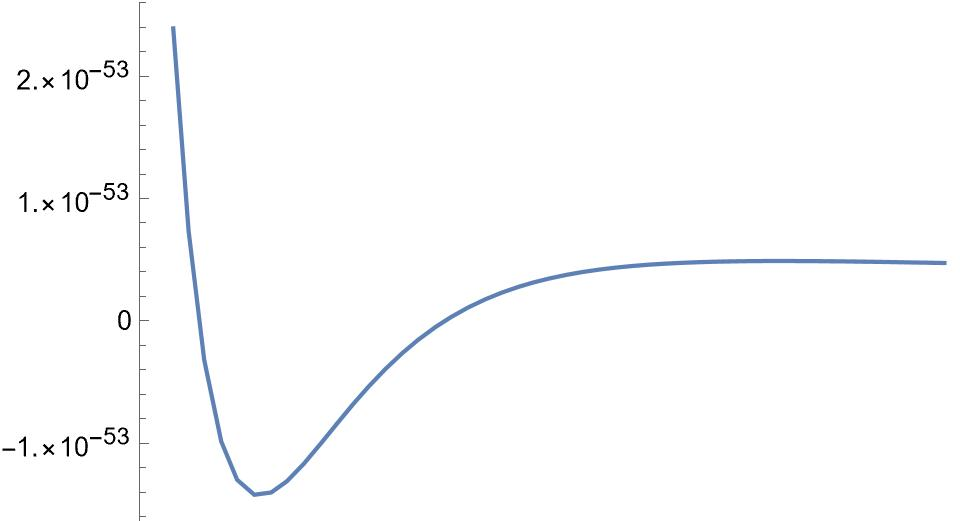
\includegraphics[keepaspectratio,width=0.6\linewidth]{fig/reference_point/plomyi_kklt.jpg}
  \end{figure}
    \begin{gather}
      w_{0}=10^{-26}, A=2, B=-10^{-30}, a=4\pi^2, 
      \nonumber
      \\
      1.6\leq T\leq 1.8, X=0.95
      \nonumber
    \end{gather}
  
\end{frame}


\begin{frame}[plain]
  \frametitle{\thesubsection\ \subsecname}

  \uline{Polonyi-KKLTモデル$+X,T$の混合}
  \begin{center}
    $
      \displaystyle
      W
      =
      w_{0}
      -
      A
      e^{-aT}
      -
      B
      \textcolor{DarkRed}{e^{-bT}}
      X
      ,\ 
      K
      =
      -
      3\ln (\tilde{T}+\bar{\tilde{T}})
      +
      |X|^2
    $
    \begin{figure}
      \centering
      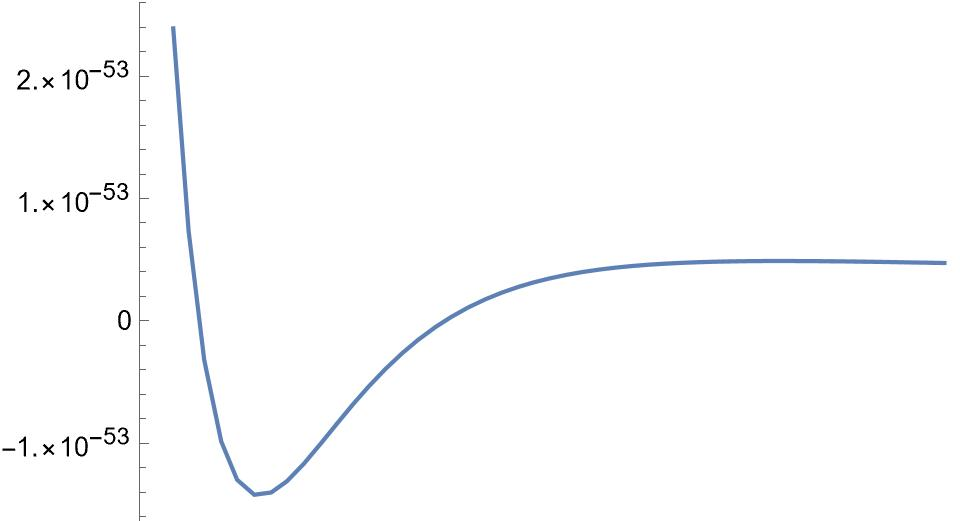
\includegraphics[keepaspectratio,width=0.6\linewidth]{fig/reference_point/plomyi_kklt_mixing.jpg}
    \end{figure}
    \begin{gather}
      w_{0}=10^{-26}, A=2, B=-10^{-30}, a=4\pi^2, b=4\pi^2
      \nonumber
      \\
      1.6\leq T\leq 1.8, X=0.95
      \nonumber
    \end{gather}
  \end{center}

\end{frame}


\begin{frame}[plain]
  \frametitle{\thesubsection\ \subsecname}

  \uline{Polonyi-KKLTモデル$+X,T$の混合}
  \begin{center}
    $
      \displaystyle
      W
      =
      w_{0}
      -
      A
      e^{-aT}
      -
      B
      \textcolor{DarkRed}{e^{-bT}}
      X
      ,\ 
      K
      =
      -
      3\ln (\tilde{T}+\bar{\tilde{T}})
      +
      |X|^2
    $
    \begin{figure}
      \centering
      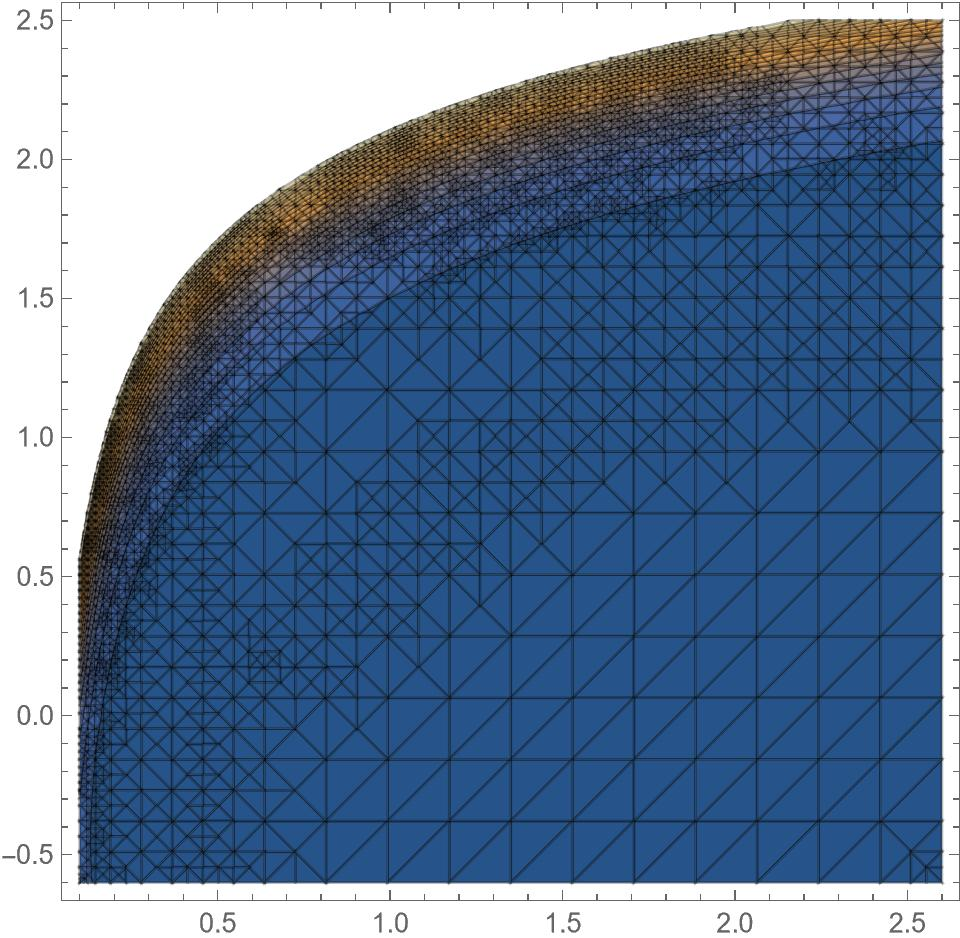
\includegraphics[keepaspectratio,width=0.3\linewidth]{fig/reference_point/plomyi_kklt_mixing_fault_contour.jpg}
      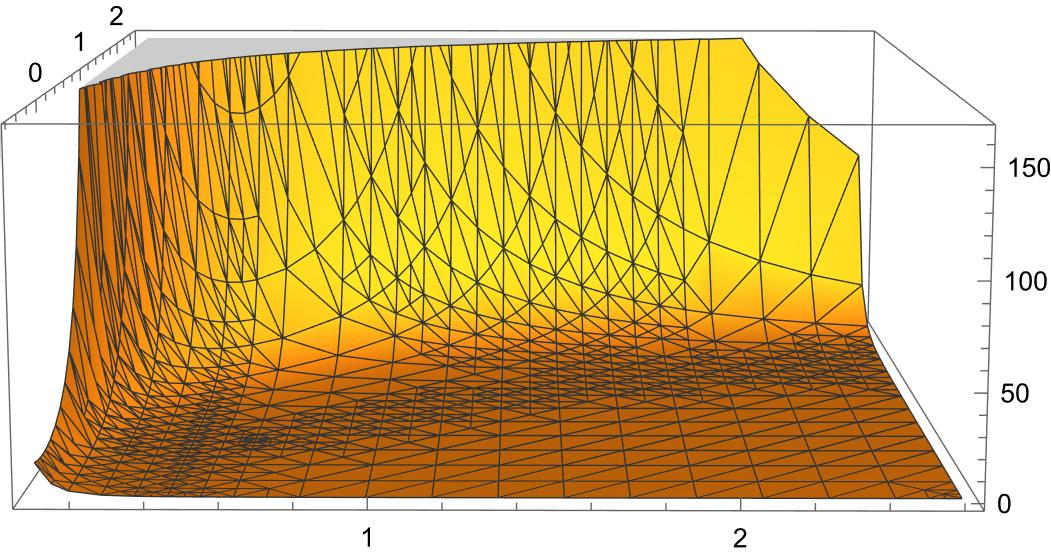
\includegraphics[keepaspectratio,width=0.3\linewidth]{fig/reference_point/plomyi_kklt_mixing_fault_3d.jpg}
      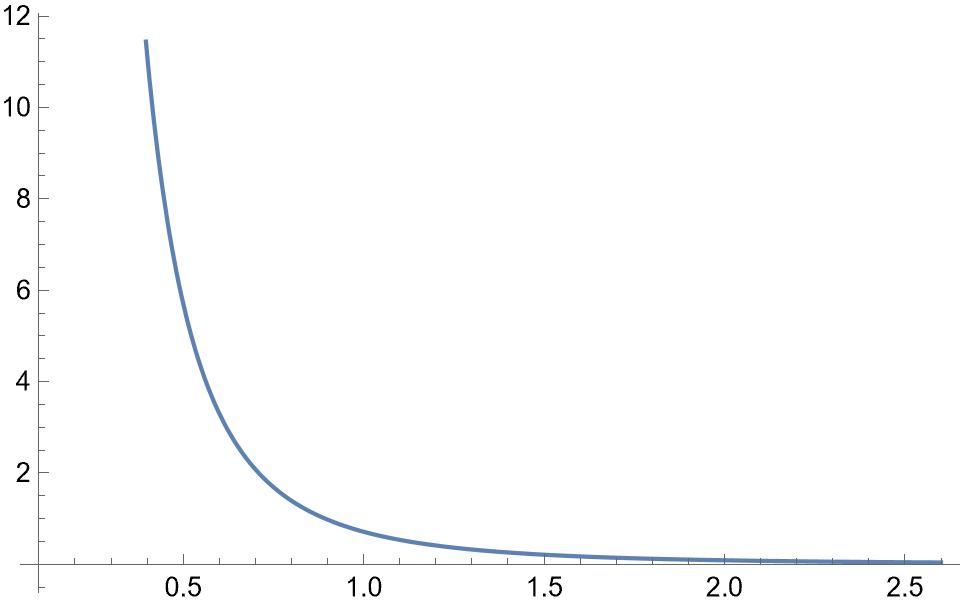
\includegraphics[keepaspectratio,width=0.3\linewidth]{fig/reference_point/plomyi_kklt_mixing_fault_plot.jpg}
    \end{figure}
    \begin{gather}
      w_{0}=10^{-26}, A=2, B=-0.5, a=4\pi^2+30, b=4\pi^2
      \nonumber
      \\
      0.1\leq T\leq 2.6, X=0.95
      \nonumber
    \end{gather}
  \end{center}

\end{frame}


% \subsection{***}

% \begin{frame}[plain]
%   \frametitle{\thesubsection\ \subsecname}







  
% \end{frame}


\setcounter{framenumber}{\value{Appendix}}
\end{document}
